% University Assignment Title Page 
% LaTeX Template
% Version 1.0 (27/12/12)
%
% This template has been downloaded from:
% http://www.LaTeXTemplates.com
%
% Original author:
% WikiBooks (http://en.wikibooks.org/wiki/LaTeX/Title_Creation)
%
% License:
% CC BY-NC-SA 3.0 (http://creativecommons.org/licenses/by-nc-sa/3.0/)
% 
% Instructions for using this template:
% This title page is capable of being compiled as is. This is not useful for 
% including it in another document. To do this, you have two options: 
%
% 1) Copy/paste everything between \begin{document} and \end{document} 
% starting at \begin{titlepage} and paste this into another LaTeX file where you 
% want your title page.
% OR
% 2) Remove everything outside the \begin{titlepage} and \end{titlepage} and 
% move this file to the same directory as the LaTeX file you wish to add it to. 
% Then add \input{./title_page_1.tex} to your LaTeX file where you want your
% title page.
%
%%%%%%%%%%%%%%%%%%%%%%%%%%%%%%%%%%%%%%%%%
%\title{Title page with logo}
%----------------------------------------------------------------------------------------
%	PACKAGES AND OTHER DOCUMENT CONFIGURATIONS
%----------------------------------------------------------------------------------------

\documentclass[12pt]{report}
\usepackage[english]{babel}
\usepackage[utf8x]{inputenc}
\usepackage{amsmath}
\usepackage{url}
\usepackage{graphicx}
\usepackage{listings}
\usepackage{afterpage}
\usepackage{eurosym}
\usepackage[colorinlistoftodos]{todonotes}
\setcounter{secnumdepth}{5}
\usepackage{cite}

\newenvironment{dedication}
  {
\clearpage           % we want a new page
   \thispagestyle{empty}% no header and footer
   \vspace*{\stretch{1}}% some space at the top 
   \itshape             % the text is in italics
   \raggedleft          % flush to the right margin
  }
  {\par % end the paragraph
   \vspace{\stretch{3}} % space at bottom is three times that at the top
   \clearpage           % finish off the page
  }

\begin{document}

\begin{titlepage}

\newcommand{\HRule}{\rule{\linewidth}{0.5mm}} % Defines a new command for the horizontal lines, change thickness here

\center % Center everything on the page
 
%----------------------------------------------------------------------------------------
%	HEADING SECTIONS
%----------------------------------------------------------------------------------------

\textsc{\LARGE Universitat Politècnica de Catalunya}\\[2.5cm] % Name of your university/college
\textsc{\Large Bachelors in Computer Science and Engineering}\\[0.5cm] % Major heading such as course name
\textsc{\large Minor Heading}\\[0.5cm] % Minor heading such as course title

%----------------------------------------------------------------------------------------
%	TITLE SECTION
%----------------------------------------------------------------------------------------

\HRule \\[0.4cm]
{ \huge \bfseries Graph and matrix algorithms for visualizing high dimensional data}\\[0.4cm] % Title of your document
\HRule \\[1.5cm]
 
%----------------------------------------------------------------------------------------
%	AUTHOR SECTION
%----------------------------------------------------------------------------------------

\begin{minipage}{0.4\textwidth}
\begin{flushleft} \large
\emph{Director:}\\
Dr. Ricard Gavalda Mestre 
\end{flushleft}
\end{minipage}
~
\begin{minipage}{0.4\textwidth}
\begin{flushright} \large
\emph{Co-Director:} \\
Dr. Marta Arias Vincente % Supervisor's Name
\end{flushright}
\end{minipage}\\[2cm]

\begin{minipage}{0.4\textwidth}
\begin{flushleft} \large
\emph{Bachelors Thesis of :}\\
Abhinav Shankaranarayanan Venkataraman
\end{flushleft}
\end{minipage}

% If you don't want a supervisor, uncomment the two lines below and remove the section above
%\Large \emph{Author:}\\
%John \textsc{Smith}\\[3cm] % Your name

%----------------------------------------------------------------------------------------
%	DATE SECTION
%----------------------------------------------------------------------------------------
\bigskip
\bigskip
{\large June 27,2016}\\[2cm] % Date, change the \today to a set date if you want to be precise

%----------------------------------------------------------------------------------------
%	LOGO SECTION
%----------------------------------------------------------------------------------------


\includegraphics{logo.png}\\[1cm] % Include a department/university logo - this will require the graphicx package
 
%----------------------------------------------------------------------------------------

\vfill % Fill the rest of the page with whitespace

\end{titlepage}

\newpage




\begin{dedication}
To my Mother, Father, Professors and Friends. I owe a lot to My professors Ricard Gavalda and Marta Arias and to Babaji at Gurudwara
\end{dedication}
\newpage
\clearpage
\newpage
\newpage

\begin{abstract}
Motivated by the problem of understanding data from
the medical domain, we consider algorithms for visually representing 
highly dimensional data so that "similar" entities appear close together. We will study, 
implement and compare several algorithms based on graph and on matrix
representation of the data. The first kind are known as "community detection"
algorithms, the second kind as "clustering" algorithms. The implementations
should be robust, scalable, and provide a visually appealing representation
of the main structures in the data.

\end{abstract}

\newpage
\clearpage
\newpage
\section*{Acknowledgement}
I would like to Acknowledge the support provided by my faculty and admins at my home university -- SASTRA University, Thanjavur and UPC Barcelona for supporting me throughout the project.

\newpage

\tableofcontents
\newpage

\chapter{Introduction}

\section{Introduction}
\setcounter{page}{1}
\par In this section	we provide an overview of the entire work. We mention the context of the project we have studied, approaches that we have used, goal of the project. We also provide the intended planning, economic estimate and sustainability of the work that has been done.


\subsection{Context Of the Project}
\par In the present day scenario, the modern science of algorithms and graph theory has brought significant advances to our understanding of complex data. Many complex systems are representable in the form of graphs. Graphs have time and again been used to represent real world networks. One of the most pertinent feature of graphs representing real system is community structures or otherwise known as clusters. Community can be defined as the organization of vertices in groups or clusters, with many edges joining the vertices of the same cluster and comparatively fewer vertices joining the vertices in another neighbouring cluster. Such communities form an independent compartment of a graph exhibiting similar role.
Thus, Community detection is the key for understanding the structure of complex graphs, and ultimately educe information from them.

\par Everyday, the number of chronic and complex patients and diseases in the health system keeps
increasing by multiple folds. In the current scenario, a patient does not have one disease but a
set of diseases. For Example a person with diabetes has a heart disease, kidney disease, blood
pressure etc. This may vary between sexes, ages etc and thus is a very complex landscape to
explore. Visualizing this landscape of diseases would help to analyse the source, the treatment
and even the path way of research to done. Thus, such a visualization would be helpful for the
medical experts and health planner to understand the landscape of diseases much better.
\par Driven by this problem of understanding data from the medical domain, the project would consider algorithms for visualizing high dimensional data so that "similar" entities called
communities are close together. Hence, we address this visualization of such high dimensional data using the algorithms and visualization technologies. All the solutions that are possible to resolve the problem will be analysed and the best solution will be determined. The project will also involve study of various algorithms and their respective analysis based on the quality and quantity of data using multiple appropriate experiments. 
\subsection{Approaches}
In this section we discuss the various approaches that are involved in dealing with the input to the project for community identification, for clustering and for visualization purposes. 
\subsubsection{For Community Identification}
Virtually in every scientific field dealing with empirical data, primary approach to get a first impression on the data is by trying to identify groups having "similar" behaviour in data. There are numerous methods to achieve this objective of which 

\begin{itemize}
\item Community Detection
\item Clustering
\end{itemize}

\paragraph{Community Detection}
\paragraph{Definition of a Community}
Communities are a part of the graph that has fewer ties with the rest of the system. Community detection traditionally focuses on the graph structures while clustering algorithms focuses on node attributes. 

Several tyoes of community detection algorithms can be distinguished
\paragraph{Divisive algorithms}
Divisive algorithms detect inter-community links and remove them from the network

\paragraph{Agglomerative algorithms}
Agglomerative algorithm merges similar nodes or communities in a recursive manner.

\paragraph{Optimization Methods}
Optimization methods are mainly based on maximization of an objective function.




\subsubsection{Clustering}

Traditional Clustering Methods are as follows:
\begin{itemize}

\item Graph Partitioning 

\item Hierarchical Clustering

\item Partitional Clustering

\item Spectral Clustering

\end{itemize}

\paragraph{Graph Partitioning}
 A typical problem in graph partitioning is the division of a set of tasks between the processors of a parallel computer so as to minimize the necessary amount of interprocessor communication.
 \par In such an application the number of processors is usually known in advance and at least an approximate figure for the number of tasks that each processor can handle. Thus we know the number and size of the groups into which the network is to be split. Also, the goal is usually to find the best division of the network regardless of whether a good division even exists; there is little point in an algorithm or method that fails to divide the network in some cases.\cite{newman2006modularity}

\paragraph{Hierarchical Clustering}
Hierarchical clustering aims to identify groups of vertices with high similarities. It can be calssifies into two categories:
 \begin{enumerate}
\item \textit{Agglomerative algorithm} : in one in which Agglomerative algorithms, in which clusters are iteratively merged if their similarity is sufficiently
high
\item \textit{Divisive algorithms}, in which clusters are iteratively
split by removing edges connecting vertices with
low similarity.
\end{enumerate} 

\paragraph{Partitional Clustering}

\paragraph{Spectral Clustering}





\subsubsection{For  Visualization}
Graph visualization is a important task in various scientific application. Visualization of data as graphs Visualizing these data
as graphs provides the non-experts with an intuitive means
to explore the content of the data, identify interesting patterns,
etc. Such operations require interactive visualizations
(as opposed to a static image) in which graph elements are
rendered as distinct visual objects; e.g., DOM objects in a
web browser. This way, the user can manipulate the graph
directly from the UI, e.g., click on a node or an edge to
get additional information (metadata), highlight parts of the
graph, etc. Given that graphs in many real-world scenarios
are huge, the aforementioned visualizations pose significant
technical challenges from a data management perspective

\paragraph{Web UI and Time per Query}
\begin{enumerate}
\item \textit{Program execution and Computation} : 
\item \textit{Building the JSON Object}
\item \textit{Communication Time}
\item \textit{Rendering }
\end{enumerate}
The total time is the sum of all the above times. 
\subsubsection{Computational Complexity}
 The estimate of the amount of resources required for by the algorithm to perform a task is defined as computational complexity. The humongous amount of data on the real graphs or real networks that are available in the current scenario causes the efficiency of the clustering algorithm to be crucial.
\par In a brief, Algorithms that have polynomial complexity describe the Class \textbf{P}. Problems whose solutions can be verified in a polynomial time span the class \textbf{NP} of \textit{non--deterministic polynomial time} problems, which includes \textbf{P}. problem is \textbf{NP}-hard if a solution for it can be
translated into a solution for any \textbf{NP}-problem. However,
a \textbf{NP}-hard problem needs not be in the class \textbf{NP}. If it
does belong to \textbf{NP} it is called \textbf{NP}-complete. The class
of \textbf{NP}-complete problems has drawn a special attention
in computer science, as it includes many famous problems like the Travelling Salesman, Boolean Satisfiability
(\textbf{SAT}), Linear Programming, etc.
The fact that \textbf{NP} problems have a solution which is verifiable in polynomial
time does not mean that NP problems have polynomial
complexity, i. e., that they are in \textbf{P}. In fact, the question of whether \textbf{NP}=\textbf{P} is the most important open problem in theoretical computer science. \textbf{NP}-hard problems
need not be in \textbf{NP} (in which case they would be \textbf{NP}-complete), but they are at least as hard as \textbf{NP}-complete
problems, so they are unlikely to have polynomial complexity, although a proof of that is still missing.
\par Many clustering Algorithms or problems related to clustering are \textbf{NP}-hard. This makes it irrelavant to use the exact algorithm, in which case we use an approximation algorithm. Approximation algorithm are methods that do not deliver the exact solution but an approximate solution but with an advantage of lower complexity. \cite{communitypaper}

\subsection{Goal of the Project}
The ability to detect groups or communities can be significant practical importance for example, a groups of world wide web (WWW) can lead to web pages on related topics, group of social network can correspond to social units or communities that share common interest.Simply finding that a graph contains tightly knit groups at all can convey useful information if a metabolic network were divided into such groups, for instance, it could provide evidence for a modular view of the network's dynamics, with different groups of nodes performing different functions with some degree of independence. There are two tempting methods that have a long history of being studied. One is graph partitioning and the other one being hierachycal cluster. Both these domains address the same question of spliting a task into communities.

\subsection{Planning}
\subsubsection{Task Description}
The tasks for the project have been subdivided into various task phases which are enumerated below : 
\begin{itemize}
\item \textbf{Required knowledge acquisition}\\
Before any immersion into the real topic, it was necessary to acquire the knowledge
necessary to understand the problem. In this phase we familiarize with the term
modularity, Louvain algorithm for community detection and various other algorithms
used for community detection.
Acquisition of knowledge about visualization tools to be used and make conversant with python is also
required.
\item \textbf{Paper Analysis}\\ In this phase we analyze and compare several works about
community detection and clustering algorithm over high dimensional graph-like data.
Doing this we became conscious of functionalities that our proposal should have and we
are thus able to guide all the subsequent phases.

\item \textbf{Design and Implementation} \\ In this phase the project is designed and coded implementing all the functionalities of the solution. 
\item \textbf{Testing I}\\
In this phase we test the program in order to identify errors in
the implementation. It includes the successive recoding.
\item \textbf{Testing II}\\
In this phase we perform tests over synthetic and real data
streams. We evaluate the performance of the program and we study
the effects of concept drift.
\item \textbf{Report Writing}\\
In this phase the report of the project is written.
\end{itemize} 
\subsection{Economic Budget}
\subsubsection{An Introduction to Economic Budget}
Economic management is primarily based on an estimate of income and expenditure called as
budget. Development of a sustainable budget leads to proper economic management of the
project. Budget and sustainability is one of the most important phase of the project
management. In this phase we analyze the budget for the project. We also aim at providing an
estimate of the project budget and optimize the same. We look at the expenditure from various
aspects such as software costs, hardware costs, license costs and human resource costs.
Additionally we also account the software for its sustainability. One important factor to note is
that the budget that we describe in this section is subject to change and it may increase
depending on the unexpected obstacles that we may face. For an instance when we don’t get
the expected results with a particular software we may have to go in for another software that
may incur extra installation and operational charges.
\subsubsection{Estimation of Economic Budget}
We divide the overall expenditure into three categories namely hardware, software and human
resources. One very important factor that we need to consider is that we only get an estimate
of the total cost. This may vary depending on the systems in use. To calculate the amortization
we consider to factors namely, first the overall life of the hardware or software in use. Second
that the project is completed in 5 months. Hence the amortization cost comes one eighth
of the actual life of the component.

\paragraph{Hardware Budget} Hardware budget accounts for the actual and the amortized costs of the hardware elements
used by the project. The cost is fictitious as it has not been developed commercially. Table 1
intents to estimate the economic cost of each of the hardware component of the project.
\\\\
\begin{tabular}{|p{1cm}||p{3cm}|p{2cm}|p{3cm}|p{3cm}|}
 \hline
 \multicolumn{5}{|c|}{Table 1 - Hardware Budget} \\
 \hline
 Sno: & Hardware Component&Useful Life &Total Cost(in \euro) &Amortized Cost(in \euro)\\
 \hline
1   & PC System  &4 &  1000\euro  & 125 \euro \\
\hline
\hline
   & \textbf{Total}  &  &  \textbf{1000}\euro  & \textbf{125} \euro \\
 \hline
\end{tabular}

\paragraph{Software Budget}
The software budget shows an estimate for the various software used in the project along with
the estimate of the software costs. It is a myth that the software doesn’t get old with time just
as a software gets but it wears out with time. Thus for every software there is a fixed time
during which it gives maximum performance. In addition freeware software and open source
software incur no cost. The cost is fictitious as it has not been developed commercially. Table 2
intents to estimate the economic cost of each of the software component of the project.
\\ \\
\begin{tabular}{|p{1cm}||p{3cm}|p{2cm}|p{3cm}|p{3cm}|}
 \hline
 \multicolumn{5}{|c|}{Table 2 - Software Budget} \\
 \hline
 Sno: & Software Component&Useful Life &Total Cost(in \euro) &Amortized Cost(in \euro)\\
 \hline
1   & Linux OS  &5 &  0\euro  & 0 \euro \\
2   & JavaScript Engine  &1 &  0\euro  & 0 \euro \\
3   & Python Components  &1 &  0\euro  & 0 \euro \\
4   & Web.py  &1 &  0\euro  & 0 \euro \\
5   & TexMaker  &1 &  0\euro  & 0 \euro \\

\hline
\hline
   & \textbf{Total}  &  &  \textbf{0}\euro  & \textbf{0} \euro \\
 \hline
\end{tabular}
\\ \\ 
\paragraph{Human Resource Budget}
The human resource budget deals with the overall expenditure spent on human resources.
Every phase of the project has a cost associated with it in per hour calculation.
The cost is fictitious as it has not been developed commercially. Table 3 intents to estimate the
economic cost of each of the phases of the project. The cost per hour is intended as an
approximation of the current cost per work hour of young analysts and developers in our
environment.\\

\begin{tabular}{|p{0.8cm}||p{4cm}|p{2.5cm}|p{1cm}|p{1.5cm}|p{2cm}|}
 \hline
 \multicolumn{6}{|c|}{Table 3 - Human Resource Budget} \\
 \hline
 Sno: & Phase&Deadline &Hours &Cost(per hour in \euro)&Total(in \euro)\\
 \hline
1   & Required Knowledge Acqusition  &1 Mar 2016 &  70  & 15\euro/h & 1050 \euro \\
2   & Paper Analysis  &1 Apr 2016& 150 &  15\euro/h  & 2250 \euro \\
3   & Design and Implementation&30 Apr 2016 &230&  20\euro/h  & 4600 \euro \\
4   & Testing I  &15 May 2016&75 &15\euro/h  & 0 1125\euro \\
5   & Testing II  &31 May 2016&75 &  15\euro/h  & 0 1125\euro \\
6   & Report Writing  &15 Jun 2016&100 &  15\euro/h  & 1500\euro \\
\hline
\hline
   & \textbf{Total}  &  & \textbf{600}&   & \textbf{10525} \euro \\
 \hline
\end{tabular}

\paragraph{Total Budget}
The following table, Table 4, summarizes the total budget for the project. This encompasses the
hardware, software and human resources budget.
\\ \\ 
\begin{tabular}{|p{1cm}||p{4cm}|p{3cm}|}
 \hline
 \multicolumn{3}{|c|}{Table 4 - Total Budget} \\
 \hline
 Sno: &Resource &Total Cost(in \euro) \\
 \hline
 1   & Hardware Budget  & 1000 \euro \\
 2   & Software Budget  & 0 \euro \\
 3   & Software Budget  & 10525 \euro \\
 \hline
\hline
   & \textbf{Total}  & \textbf{11525} \euro \\
 \hline
 
 

\end{tabular}


\subsection{Sustainability}
Sustainability is a key factor in any project design. We evaluate the project based on three
factors of sustainability namely economic sustainability, social sustainability and environmental
sustainability.
\subsubsection{Economic Sustainability}
 In this document we specify
the budget estimation of the project. From our estimation it can be said that this will be the
maximum bound on the budget for the project. This takes into account all the factors namely
the hardware costs, software costs and human resource costs. The cost estimated in the project is the least possible cost and hence is a nonpareil project estimate for any indistinguishable project. The budget
may exceed our calculations only during unexpected times. When the proposed plan is precisely followed the estimated lower costs gets achieved. 
Also the product that we aim at developing here is tested with all kinds of data and we aim at
building a very high quality software which in turn provides a durable software that will not
wear out easily.  Most of the software used in the project is open source which has zero product cost. The The hardware required is nothing but computers that becomes a mandatory part
of any project in the present days.

\subsubsection{Social Sustainability}
The project aims at developing web based platform to perform learning cum visualization
analytics. This is indirectly going to analyze the learning characteristics of the patients and
provide a feedback both to the medical analyzer and health planner. This is going to improve
the quality of health analysis in the state. All this requires is a simple computer connected to
the internet. This has very keen social motive and this project when completed is going to
improve the standard of learning in schools. Thus this has a great social responsibility. This is in
turn justifies why this project has a great social sustainability.

\subsubsection{Environmental Sustainability}
From the sections of temporal planning and the budget planning we understand that we have a
computer running throughout the project. If we make an assumption that the amount of
energy used by a single computer comes to around 250 watts. And given that we spend 500
hours on the project then the energy expended is 125KW. This amounts to 48.125 kg of
$CO_2$ . This is indeed a high amount but well within the permissible limits. This can be reduced
by reducing the code size which is possible by reusing the already existing code. But the project
is actually environmentally sustainable.

\chapter{Background Knowledge}
\section{Introduction}
In this section we present the background knowledge required to understand and solve the problem
\subsection{Graph Notation}

\subsubsection{Graph Definition}
Graph ,\textit{G} , is construct consisting of two finite sets, the set \textit{V} = \{ $v_1,v_2, \ldots ,v_n$ \} of vertices and the set \textit{E} = \{ $e_1,e_2, \ldots,e_n$  \} of edges where each edge is a pair of vertices from \textit{V}, for instance,
\begin{center}
$e_i = (v_j,v_k)$
\end{center}
is an edge from $v_j$ to $v_k$ represented as \textit{G}=(\textit{V},\textit{E}). In other words  E $\subset V^2$, which is the set of all unordered. The vertices ($v_j$ and $v_k$) that represent an edge are called \textit{endpoints} and the edge is said to be adjacent to each of its end points.  \cite{PeterLinz}

\begin{figure}[h]
\caption{Example Graph G=(V,E) Bull Graph}
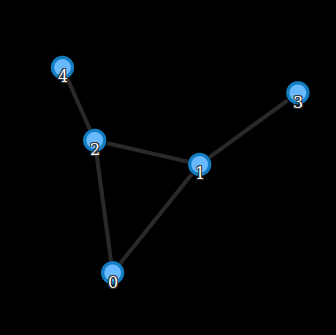
\includegraphics[scale=0.5]{bull.png}
\centering
\end{figure}

The neighbourhood of a node $v_i$ is the set of
nodes $v_i$ is connected to, N($v_i$) = $\{v_j | (v_i, v_j) \in E, v_i \neq
v_j, 1 \leq j \leq n\}$. The degree of a node vi, or the size of
the neighborhood connected to $v_i$, is denoted as d($v_i$) =
$|N(v_i)|$. 
\par A degree sequence, \textit{D}, specifies the set of all node
degrees as tuples, such that D = {($v_i, d(v_i)$} and follows a
probability distribution called the \textit{degree distribution} with
mean $d_m$. \cite{githubtest1}

\subsection{Graph Matrix Notation}
Graphs can be appropritely represented in the form of matrices for instance, adjacency matrix, admittance matrix etc.,
\\
Let \textit{G}=(\textit{V},\textit{E}) be a simple graph with vertex set \textbf{V} and edge set \textbf{E}, then the adjacency matrix is square $|V|^2$ matrix \textbf{M} such that its element $M_{i,j}$ is \textit{1} when there is an edge from $v_i$ to $v_j$,where $v_i \in \textbf{V}$ , $ v_j \in \textbf{V}$ and \textit{0} when there is no edge.
The adjacency matrix of a graph of order \textit{n} entitles the entire the topology of a graph.  The diagonal elements of the adjacency matrix are all \textit{0} for undirected graphs \textbf{M}.
\par The sum of the elements of \textit{i}-th row or column yields the degree of node \textit{i}. If the edges are weighted, one defines the weight matrix \textbf{W}, whose element \textit{W}$_{ij}$ expresses the weight of the edges between vertices \textit{i} and \textit{j}.

\par The \textit{spectrum} of a graph \textbf{G} is the set of eigenvalues of it's adjacency matrix \textbf{M}. If \textbf{D}  is the diagonal matrix whose element \textit{D} $_{i,i}$ equals the degree of vertex i ($v_i \in$ \textit{V}).



\subsection{State-of-the-art in Community Detection}
Modularity is the objective function that is widely used both as a measure and as a optimzing method for partitioning community.
As said before there are various algorithms that can be used for community detection . In reference to the paper \cite{generalcommunity} which discusses 6 different community detection algorithms namely: 
\begin{itemize}
\item Louvain Method
\item Le Martelot
\item Newman’s greedy algorithm (NGA)
\item Newman’s spectral algorithm with refinement
\item simulated annealing
\item extremal optimization
\end{itemize}
The following figure the average normalized performance rank of each algorithm in terms of partitioning quality and speed. Taken from the paper that proposed Combo algorithm \cite{generalcommunity}. 
\begin{figure}[h]
\caption{Average normalized performance rank of each algorithm in terms of partitioning quality and speed}
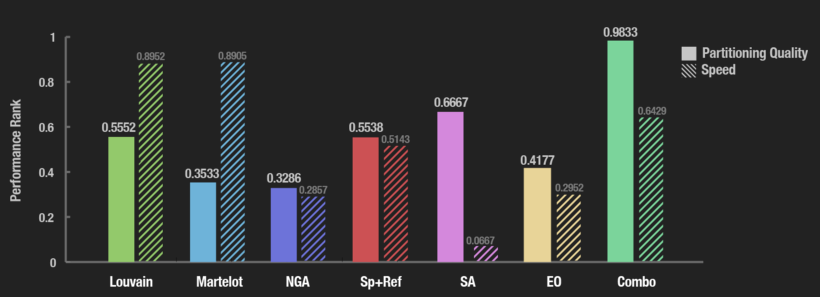
\includegraphics[scale=0.5]{lou.png}
\centering
\end{figure}
The main Objective of the project is to visuvalize the data on screen thus needs an algorithm that is fast and should be effective.  Hence louvain algorithm was choosen for the implementation. The implementation can be found in the later scection of the project.


Louvain algorithm \cite{louvain} is fast,recursive and is more effective on real world graphs. Oweing to our object of projecting medical domain we require an algorithm that gives a better trade off between being effective and being fast. Hence Louvain algoithm was choosen.


\subsection{State-of-the-art in Graph Visualization}

\chapter{Community Detection Algorithm}
\section{Introduction}
In this section we would describe the community detection algorithms such as louvain and various tests that were performed to choose the algorithm. 
\section{Louvain Algorithm}
\subsection{Introduction}

The problem of community detection requires the graph to be split into communities of tightly packed or in other words densely connected nodes with nodes of different community being sparely connected. 

Several algorithms have been proposed for perfoming good partition in a reasonably good speed.
Distinguishably there are several types of community detection algorithms, namely: divisive algorithms, which aims in removal of the inter-community links, agglomerative algorithms, which aim in merging similar nodes and optimization methods which aim in maximzing the objective function. 
\subsection{Modularity}
The quality of partitioning that results from application of method is often measured using modularity. The \textit{modularity} of a partition is hence a scalar value between -1 and 1 that is used to measure the density of the links inside the communities as compared to the density of the links between the communities.
\par
Modularity not only serves as a quality measure for detecting the quality of split or partition, but also acts as an objective function to optimize.  Exact modularity optimization is \textbf{NP-Complete} in the strong sense \cite{modularityNP}.
\subsubsection{Definition}
Let G=(V,E) be a simple graph,where \textit{V} is the set of vertices and \textit{E} is the set of undirected edges. Let $n=|V|$ and $m=|E|$. Let degree of a vertex \textit{v} be, deg(\textit{v}) where \textit{v} $\in$ V. Let C be the community, $C \subseteq V$, be the subset of vertices. A \textit{clustering} $C_s =\{C_1,C_2, \ldots, C_k\}$ of G is a partition of V such each vertex is present exactly in one cluster.  We thus define \textit{modularity } as follows: \cite{modularityNP}

\begin{equation} \label{eq1}
\begin{split}
Q(C_s) &= \sum_{C \in C_s}\left[ \frac{|E(C)|}{m} - \left( \frac{|E(C)+\sum_{k \in C_s}|E(C,k)|}{2m} \right)^2 \right]
\end{split}
\end{equation}
where E(I,J) is set of all edges between vertices in cluster I and J. E(C) = E(C,C).
The above equation can be continently rewritten as follows: 
\begin{equation} \label{eq1}
\begin{split}
Q(C_s) &= \sum_{C \in C_s}\left[ \frac{|E(C)|}{m} - \left( \frac{\sum_{v \in C}deg(v)}{2m} \right)^2 \right]
\end{split}
\end{equation}

\subsection{Implementation}

The implementation  of the algorihtm is based on the paper "Fast unfolding of communities in large networks" \cite{louvain}.  The implementation is done using basic python packages. 
 The Algorithm has two phases that are repeated iteratively to bring the final solution to the problem. The following figure(Figure 3.1) demonstrates the algorithm in the form of a flow diagram,
 \begin{figure}[h]
\caption{Visualization of the steps of our algorithm. Each pass is made of two phases:
one where modularity is optimized by allowing only local changes of communities;
one where the found communities are aggregated in order to build a new network of
communities. The passes are repeated iteratively until no increase of modularity is
possible. This was taken from the paper "Fast unfolding of communities in large networks" \cite{louvain}}
\textbf{First Phase}
Let G be a graph with N nodes in the network. The algorithm assigns a different community to each node in the network.  The number of nodes is equal to the number of communities in the graph. The report uses the terms node and vertices interchangably.  Let $v_i$ be be a node such that $v_j$ $\in$ N($v_i$). The gain of modularity is then calculated by removing $v_i$ and placing it in community of $v_j$. If the gain is positive the $v_i$ is moved to the community of $v_j$ else $v_i$ stays in it's original community. This procedure is iterated and the phase one stops when a local maxima of the modularity is achieved, that is when no more move of nodes from one community to another is possible. The ordering of the nodes can affect or effect the computation time which can be a part of furutre works. 
\par The main algorithm relies on the calculation of modularity. Listing 3.1 demonstarted the calculation using a python snippet. 

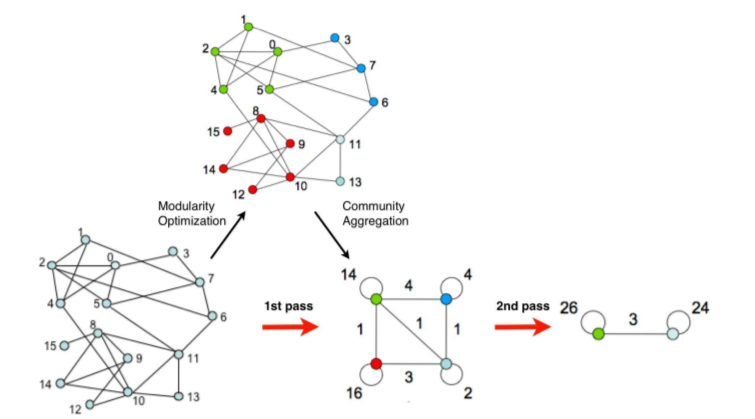
\includegraphics[scale=0.5]{loustep.png}
\centering
\end{figure}
\begin{lstlisting}[language=Python, caption=Modularity Calculation]
# a method from the louvain class. 
# The variables are as equivalent as 
# in the above formula 3.2
 def modularity_calc(self,partition):
        q = 0
        m2 = self.m * 2 
        for i in range(len(partition)):
            q += self.s_in[i] / m2 - (self.s_tot[i] / m2) ** 2
        return q
    
\end{lstlisting}
\par The first phase

\begin{lstlisting}[language=Python, caption=First Phase of Louvain]
    def first_phase(self, network):
        # make initial partition
        best_partition = self.make_initial_partition(network)
        while 1:
            improvement = 0
            for node in network[0]:
                node_community = self.communities[node]
                # default best community is its own
                best_community = node_community
                best_gain = 0
                # remove _node from its community
                best_partition[node_community].remove(node)
                best_shared_links = 0
                for e in self.edges_of_node[node]:
                    if e[0][0] == e[0][1]:
                        continue
                    if e[0][0] == node and self.communities[e[0][1]] == node_community or e[0][1] == node and self.communities[e[0][0]] == node_community:
                        best_shared_links += e[1]
                self.s_in[node_community] -= 2 * (best_shared_links + self.w[node])
                self.s_tot[node_community] -= self.e_sum[node]
                self.communities[node] = -1
                communities = {} # only consider neighbors of different communities
                for neighbor in self.get_neighbors(node):
                    community = self.communities[neighbor]
                    if community in communities:
                        continue
                    communities[community] = 1
                    shared_links = 0
                    for e in self.edges_of_node[node]:
                        if e[0][0] == e[0][1]:
                            continue
                        if e[0][0] == node and self.communities[e[0][1]] == community or e[0][1] == node and self.communities[e[0][0]] == community:
                            shared_links += e[1]
               
                    gain = self.modularity_calc_gain(node, community, shared_links)
                    if gain > best_gain:
                        best_community = community
                        best_gain = gain
                        best_shared_links = shared_links
                # insert _node into the community maximizing the modularity gain
                best_partition[best_community].append(node)
                self.communities[node] = best_community
                self.s_in[best_community] += 2 * (best_shared_links + self.w[node])
                self.s_tot[best_community] += self.e_sum[node]
                if node_community != best_community:
                    improvement = 1
            if not improvement:
                break
        return best_partition
        
\end{lstlisting}


\subsubsection{Experiments}
\cite{githubtest1}
\subsubsection{Result}

\section{Matrix Based Algorithm}
\subsection{Matrix Algorithm}
\subsubsection{Introduction}
\subsubsection{Reasoning}
\subsubsection{Description}
\subsubsection{Implementation}
\subsubsection{Experiments}
\subsubsection{Result}

\chapter{Visualization Techniques}
\section{Introduction}
\subsection{Alchemy.js}
\subsubsection{Introduction}
\subsubsection{Reasoning}
\subsubsection{Description}
\subsubsection{Methods and Library}
\subsubsection{Result}

\chapter{Overall System Description}
\section{Overall System Description}
\subsection{Web.py}
\subsubsection{Introduction}
\subsubsection{Implementation Benefits}
sdgbf akjsfkldsnfksndafnadfa
fasfadf
adfasfasfadf
asfasfadf
afadfadf
\subsubsection{Description}
git hub repository  : \url{https://github.com/abhinavsv3/webproject}
\subsubsection{Result}
\subsection{Benefits to the community}
This can be used in places where there is difficulty in visualization of a very complex landscape
of data such as medical domain. In Medical domain a patient can be a vector of diseases and
visualization of such patients (patients graph–which shows relations of how two patients are
similar, a graph in which patient-patient edge weight is the similarity value ) would be useful for
analyzing and predicting the disease landscape of a region and in turn multiple regions.

\chapter{Conclusion and Future Works}
\section{Goals Achieved}
\section{Revision of Planning and Budget}
\section{Future Works}
Order of inputs can influence the computation time. The problem of finding specific heuristics to solve this ordering problem can improve the louvain algorithms computation time.
\section{Availability and requirements}
\begin{enumerate}
\item \textbf{Project Name}: Graph and matrix algorithms for visualizing high dimensional
\item \textbf{Project Homepage}: \url{https://github.com/abhinavsv3/webproject dimensional}
\item \textbf{Operating System}: Platform Independent. Preferably Unix--like operating system
\item \textbf{Programming Language}: Python 2.7
\item \textbf{Other Requirements} : Alchemy.js, Python Packages, Web.py
\end{enumerate}

\subsection{Conclusion}
This is one of the greatest project experience.	
\subsection{Personal Conclusion}
This is one of the greatest project experience.	

\lstlistoflistings

\bibliographystyle{plain}
\bibliography{mybib}{}
\end{document}



\begin{lstlisting}[language=Python, caption=Creation of JSON Object using Python]
import json as j
from copy import deepcopy
la=[]
lb=[]
jd = {"nodes":la,"edges":lb}
# for the node 
k = {}
k['id'] = "1"
k['cluster']= "1"
k['title'] = "Abc"
k["relatedness"]="0.5"
jd['nodes'].append(deepcopy(k))
print jd
k['id'] = "2"
k['cluster']= "2"
k['title'] = "two"
k["relatedness"]="0.5"
jd['nodes'].append(deepcopy(k))

#For the Edge
m = {}
m["source"] = "1"
m["target"] =  "2"
m["relatedness"] = "0.5"
jd['edges'].append(m)

prin = j.dumps(jd,indent = 4)
print prin

f = open("crea.json","w")
f.write(prin)
f.close()
\end{lstlisting}

\begin{lstlisting}[language=Python, caption=Modularity Calculation]
# a method from the louvain class. 
# The variables are as equivalent as 
# in the above formula 3.2
 def modularity_calc(self,partition):
        q = 0
        m2 = self.m * 2 
        for i in range(len(partition)):
            q += self.s_in[i] / m2 - (self.s_tot[i] / m2) ** 2
        return q
    
\end{lstlisting}

\begin{lstlisting}[language=Python, caption=First Phase of Louvain Algorithm]
best_partition = self.make_initial_partition(network)
while 1:
    improvement = 0
    for node in network[0]:
        node_community = self.communities[node]
        # default best community is its own
        best_community = node_community
        best_gain = 0
        # remove _node from its community
        best_partition[node_community].remove(node)
        best_shared_links = 0
        for e in self.edges_of_node[node]:
            if e[0][0] == e[0][1]:
                continue
            if e[0][0] == node and self.communities[e[0][1]] == node_community or e[0][1] == node and self.communities[e[0][0]] == node_community:
                best_shared_links += e[1]
        self.s_in[node_community] -= 2 * (best_shared_links + self.w[node])
        self.s_tot[node_community] -= self.e_sum[node]
        self.communities[node] = -1
        communities = {} # only consider neighbors of different communities
        for neighbor in self.get_neighbors(node):
            community = self.communities[neighbor]
            if community in communities:
                continue
            communities[community] = 1
            shared_links = 0
            for e in self.edges_of_node[node]:
                if e[0][0] == e[0][1]:
                    continue
                if e[0][0] == node and self.communities[e[0][1]] == community or e[0][1] == node and self.communities[e[0][0]] == community:
                    shared_links += e[1]
            # compute modularity gain obtained by moving _node to the community of _neighbor
            gain = self.modularity_calc_gain(node, community, shared_links)
            if gain > best_gain:
                best_community = community
                best_gain = gain
                best_shared_links = shared_links
        # insert _node into the community maximizing the modularity gain
        best_partition[best_community].append(node)
        self.communities[node] = best_community
        self.s_in[best_community] += 2 * (best_shared_links + self.w[node])
        self.s_tot[best_community] += self.e_sum[node]
        if node_community != best_community:
            improvement = 1
    if not improvement:
        break
return best_partition

\end{lstlisting}
